% Adjust these for the path of the theme and its graphics, relative to this file
%\usepackage{beamerthemeFalmouthGamesAcademy}
\usepackage{../../beamerthemeFalmouthGamesAcademy}
\usepackage{multimedia}
\graphicspath{ {../../} }

% Default language for code listings
\lstset{language=C++,
        morekeywords={each,in,nullptr}
}

% For strikethrough effect
\usepackage[normalem]{ulem}
\usepackage{wasysym}

\usepackage{pdfpages}

% http://www.texample.net/tikz/examples/state-machine/
\usetikzlibrary{arrows,automata}

\newcommand{\modulecode}{COMP260}\newcommand{\moduletitle}{Distributed Systems}\newcommand{\sessionnumber}{5}

\begin{document}
\title{\sessionnumber: Meshes and movement}
\subtitle{\modulecode: \moduletitle}

\frame{\titlepage} 

\begin{frame}
	\frametitle{Agenda}
	\begin{itemize}
		\item Portfolio task check-in (sprint planning)
		\item Complex meshes (goodbye triangle, hello cube!)
		\item First-person camera control
	\end{itemize}
\end{frame}

\begin{frame}{Next week}
	\begin{itemize}
		\pause\item Timetable change: COMP220 lecture is on \textbf{Wednesday morning} in Seminar D
		\pause\item \textbf{Compulsory} catch-up tutorials on Tuesday 18th, in the afternoon
			\begin{itemize}
				\pause\item Book now -- if you haven't booked by Friday 5pm then I will book for you!
				\pause\item If you can't make it on Tuesday afternoon, let me know ASAP so that we can arrange another time
			\end{itemize}
	\end{itemize}
\end{frame}

\begin{frame}{Portfolio task check-in}
	\begin{itemize}
		\pause\item Please show me your \textbf{Trello board} now
		\pause\item You are now in your \textbf{first sprint}
		\pause\item Your first sprint review is \textbf{in 2 weeks}
	\end{itemize}
\end{frame}

\part{More complex meshes}
\frame{\partpage}

\begin{frame}{Winding order}
	\begin{itemize}
		\pause\item It is sometimes important to know which side of a triangle is the ``front'' and which is the ``back''
		\pause\item OpenGL determines this by \textbf{winding order}
	\end{itemize}
	\begin{columns}
		\pause
		\begin{column}{0.48\textwidth}
			\begin{center}
				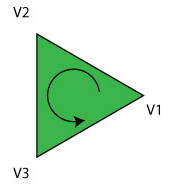
\includegraphics[width=0.5\textwidth]{winding_ccw}
				
				If the vertices go \textbf{anticlockwise}, you are looking at the \textbf{front}
			\end{center}
		\end{column}
		\pause
		\begin{column}{0.48\textwidth}
			\begin{center}
				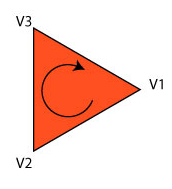
\includegraphics[width=0.5\textwidth]{winding_cw}
				
				If the vertices go \textbf{clockwise}, you are looking at the \textbf{back}
			\end{center}
		\end{column}
	\end{columns}
\end{frame}

\begin{frame}[fragile]{Backface culling}
	\pause
	\begin{lstlisting}
glEnable(GL_CULL_FACE);
	\end{lstlisting}
	\begin{itemize}
		\pause\item This will cause only the front faces of triangles to be drawn
		\pause\item Triangles whose front face is not visible will be \textbf{culled}
		\pause\item Culled faces are not passed through the rasteriser or fragment shader
		\pause\item Saves time, and should make no difference to appearance ---
			as long as all meshes are closed and have correct winding
	\end{itemize}
\end{frame}

\begin{frame}[fragile]{When backface culling goes bad?}
	\begin{center}
		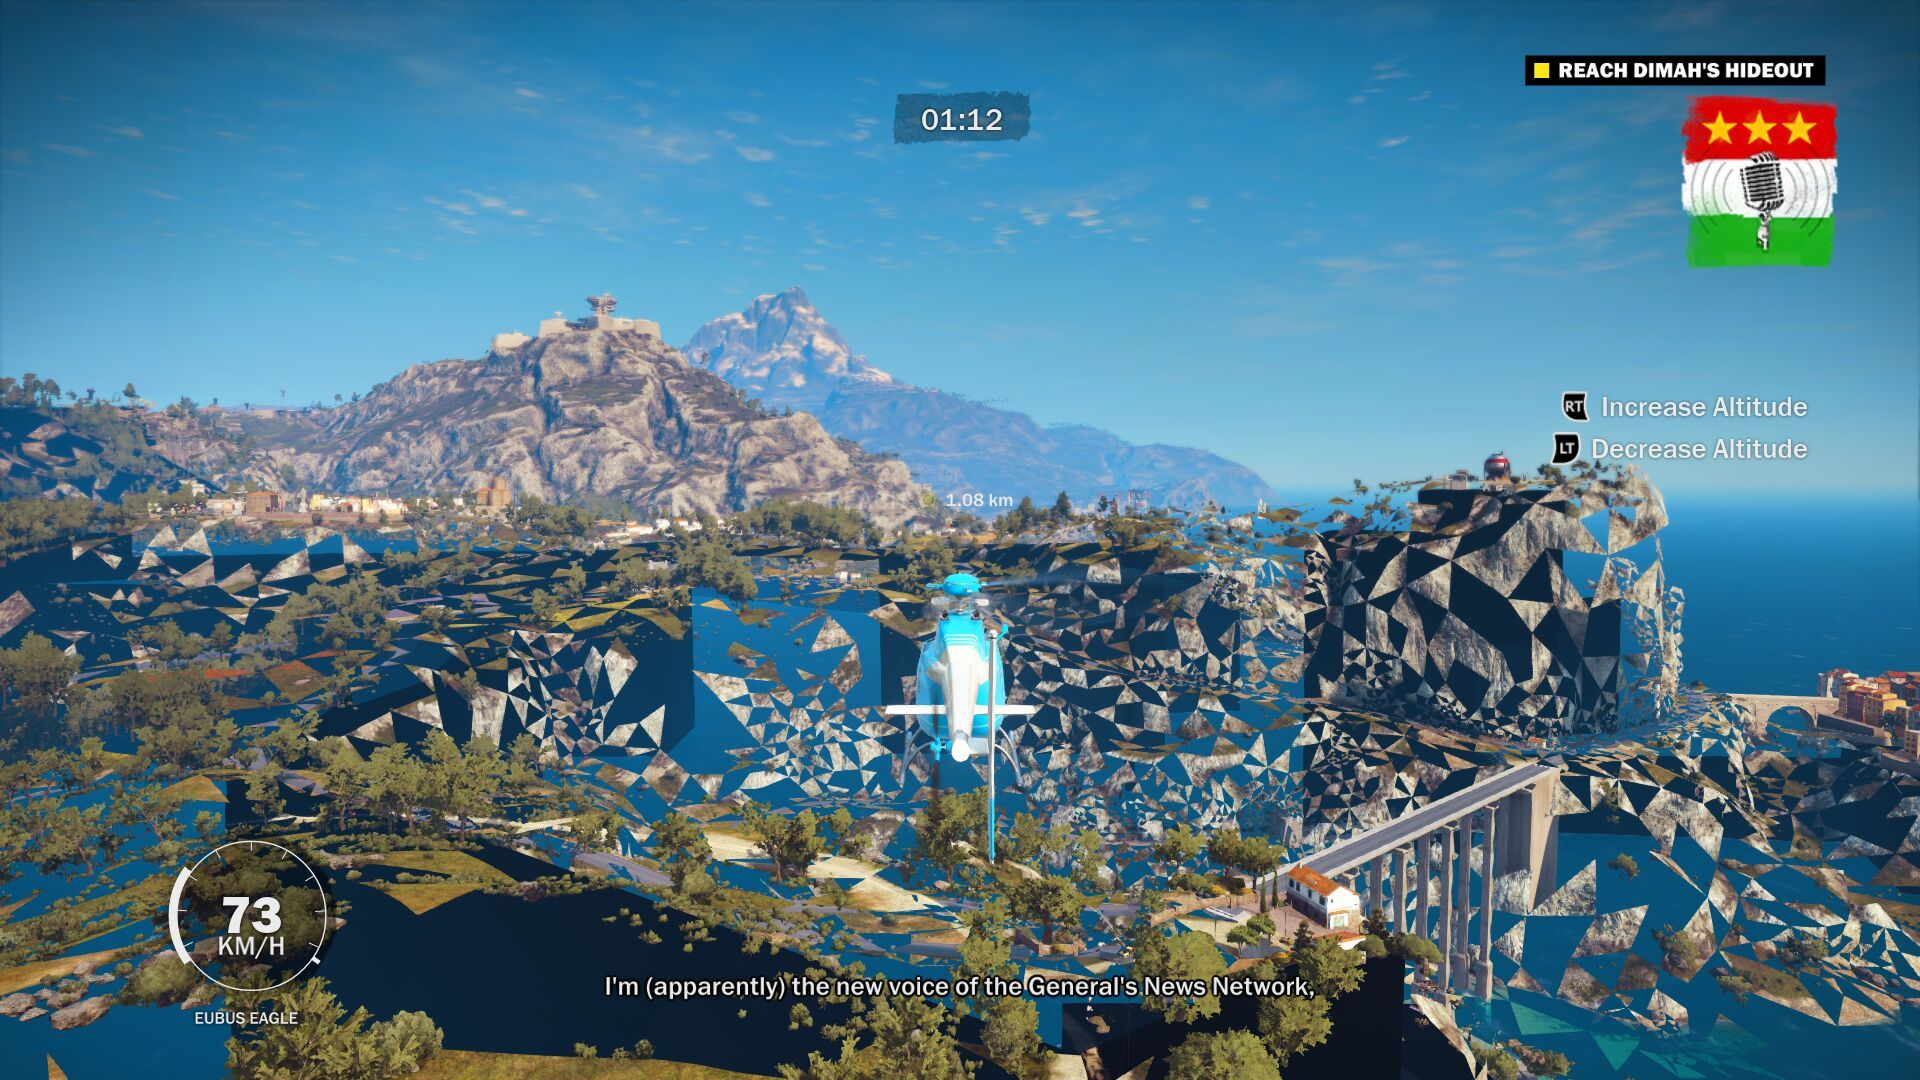
\includegraphics[width=\textwidth]{missing_triangles}
	\end{center}
\end{frame}

\begin{frame}{Let's draw a square!}
	\begin{center}
		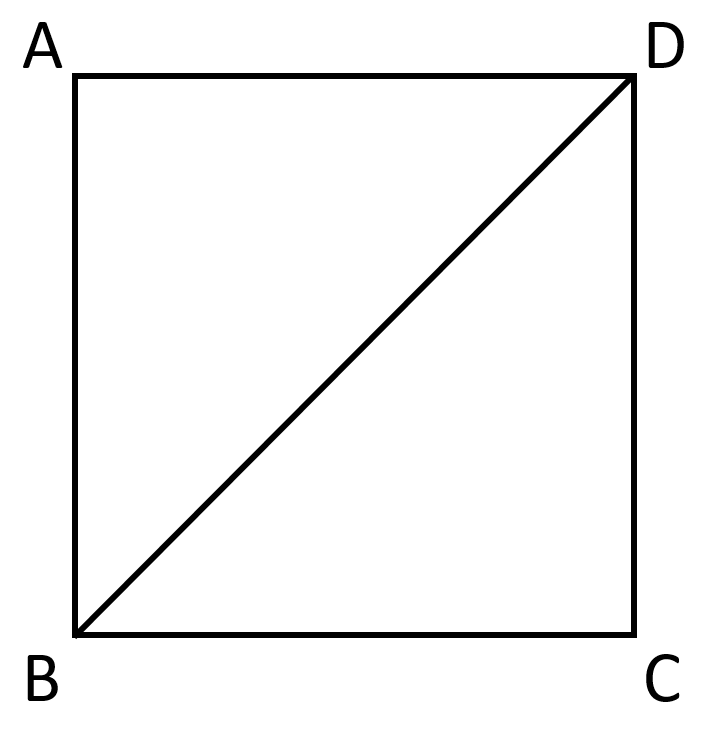
\includegraphics[height=0.8\textheight]{square_vertices}
	\end{center}
\end{frame}

\begin{frame}{Let's draw a cube!}
	\begin{center}
		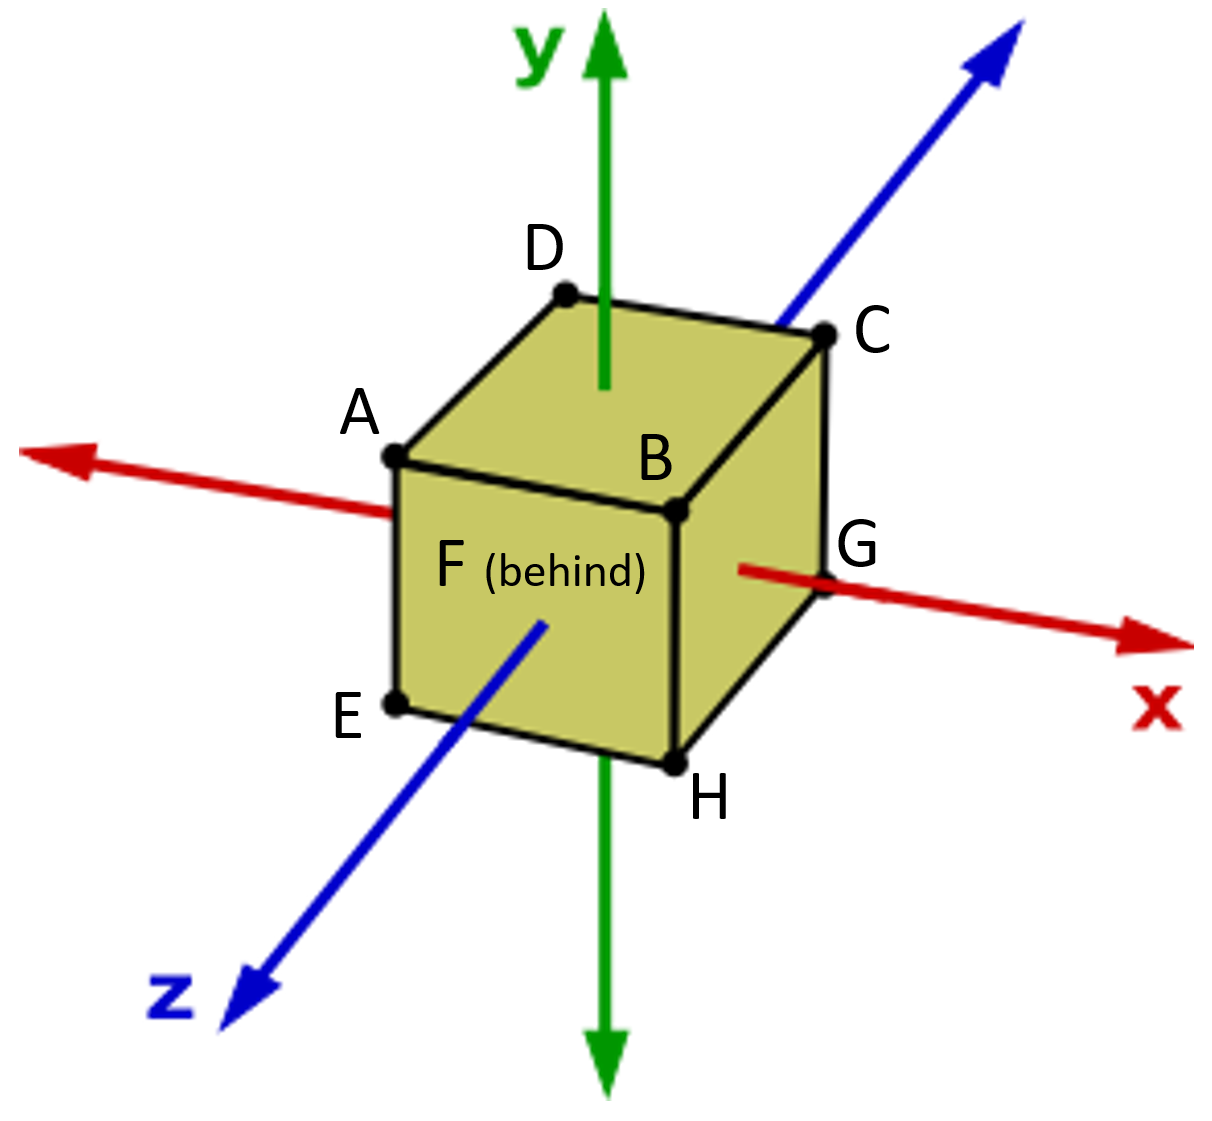
\includegraphics[height=0.8\textheight]{cube_vertices}
	\end{center}
\end{frame}


\part{First person camera control}
\frame{\partpage}

\begin{frame}{The plan}
	\begin{itemize}
		\pause\item Represent the player's \textbf{position} by a 3D vector
		\pause\item Represent the player's \textbf{orientation} by Euler angles
		\pause\item Mouse events change these angles
		\pause\item View matrix is calculated using position and orientation
		\pause\item To move forwards, use the Euler angles to find the ``forward'' vector,
			and offset the position by this vector
	\end{itemize}
\end{frame}

\begin{frame}{Keyboard and mouse in SDL}
	\pause Use \textbf{relative mouse mode}
	\begin{itemize}
		\pause\item Hides the mouse pointer
		\pause\item Prevents the mouse pointer from hitting the edge of the screen
		\pause\item Gives us the distance the mouse has moved since last frame, rather than its current position
	\end{itemize}
	\pause Use \lstinline{SDL_GetKeyboardState} instead of handling individual keyboard events
	\begin{itemize}
		\pause\item Allows us to check on every frame whether the key is held down
		\pause\item Otherwise, the player will move jerkily according to the key repeat rate
	\end{itemize}
\end{frame}

\begin{frame}{Vector addition}
	\pause
	\begin{center}
		\colorbox{white}{
			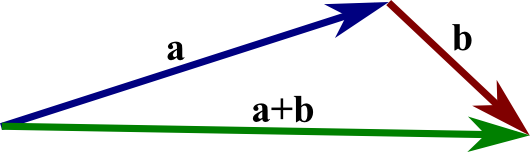
\includegraphics[width=0.5\textwidth]{vector_addition}
		}
	\end{center}
	\begin{itemize}
		\pause\item E.g.\ if $a$ is current position, and
		\pause\item $b$ is the distance and direction we want to move, then
		\pause\item $a + b$ is the new position
	\end{itemize}
\end{frame}

\begin{frame}{Addition in homogeneous coordinates}
	\begin{itemize}
		\pause\item Recall: homogeneous coordinates have an extra $w$ component, i.e.\ $(x,y,z,w)$
		\pause\item $w=1$ for positions, $w=0$ for offsets
	\end{itemize}
	\begin{tabular}{rclclc}
		\pause offset & + & offset & = & offset & $w = 0 + 0 = 0$ \\
		\pause position & + & offset & = & position & $w = 1 + 0 = 1$ \\
		\pause position & + & position & = & ??? & $w = 1 + 1 = 2$
	\end{tabular}
\end{frame}

\begin{frame}{Unit vectors}
	\begin{itemize}
		\pause\item A \textbf{unit vector} is a vector of length 1
		\pause\item I.e.\ $\sqrt{x^2 + y^2 + z^2} = 1$ (Pythagoras)
		\pause\item Useful to represent \textbf{direction}
		\pause\item Multiplying a vector of length $a$ by a number $b$ gives a vector of length $a \times b$,
			parallel to the original vector
		\pause\item So multiplying a unit vector by $b$ gives a vector of length $b$,
			parallel to the unit vector		
	\end{itemize}
\end{frame}

\begin{frame}{Representing look direction}
	\begin{columns}
		\pause
		\begin{column}{0.48\textwidth}
			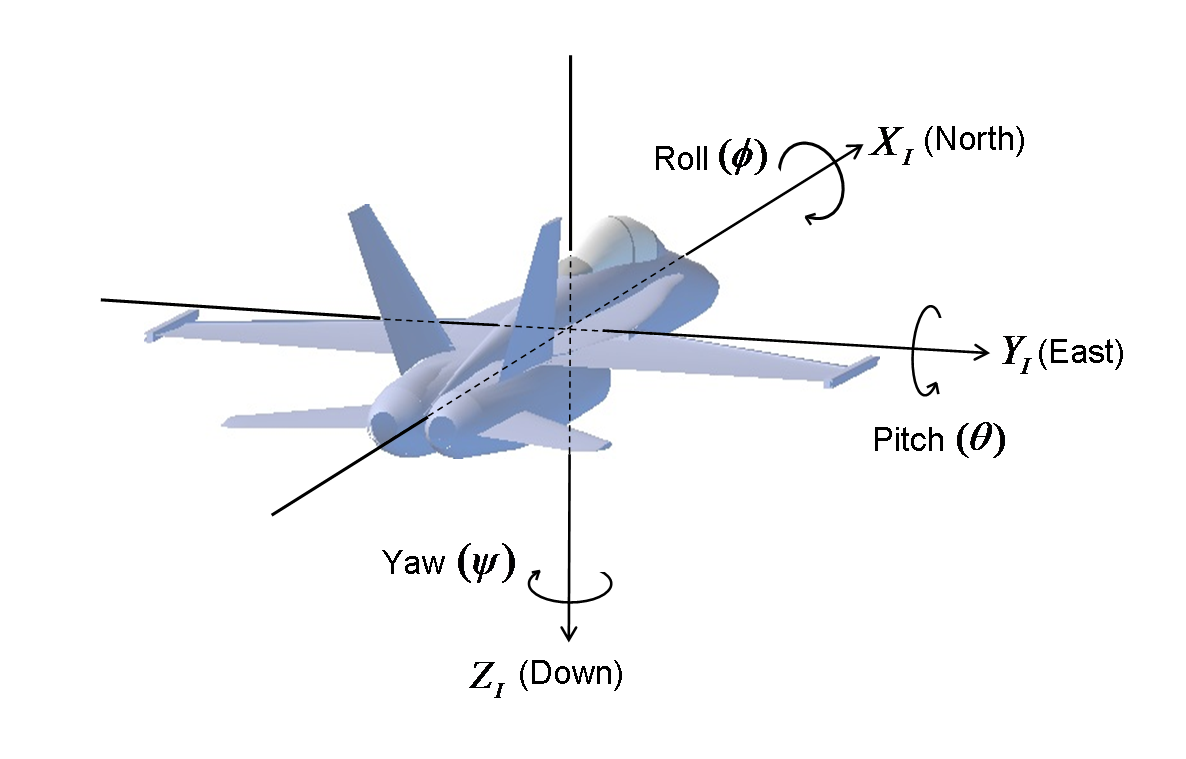
\includegraphics[width=\textwidth]{../03/euler_aeroplane}
		\end{column}
		\begin{column}{0.48\textwidth}
			\begin{itemize}
				\pause\item Euler angles
				\pause\item Don't need roll, just pitch and yaw
				\pause\item (Not using roll eliminates the gimbal lock problem)
				\pause\item Forward vector and look vector can be obtained by appropriate rotation of a unit vector
			\end{itemize}
		\end{column}
	\end{columns}
\end{frame}


\end{document}
